\documentclass[10pt,a4paper]{article}
\usepackage{amsmath}
\usepackage{graphicx}
\usepackage[margin=1in]{geometry}

\catcode`\_=\active
\def_{\_}

\begin{document}

\begin{titlepage}
\title{G52GRP Interim Group Report\\HEX - A Chain Reactive Music Generator }
\author{Group NHN2}
\date{22nd March 2013}
\maketitle
\thispagestyle{empty}
\begin{center}
Supervisor: Dr. Henrik Nilsson\\
\bigskip
\begin{tabular}{ l c r }
  S.Cooke & - & skc01u \\
  R. Fulton & - & rxf01u \\
  G. Hallam & - & goh01u \\
  D. Huo & - & dxh02u \\
  M. Tawafig & - & mxt41u \\
  J. Sherry & - & jxs41u \\  
\end{tabular}
\end{center}
\end{titlepage}

\tableofcontents
\pagebreak

\part{Preliminaries}
\section{Concept}
\subsection{ReacTogon Concept}
The \textit{`ReacTogon`}\cite{modin} is a concept instrument produced by Mark Burton in 2007. Described as a `chain-reactive performance arpeggiator', it acts as a physical user interface to a synthesiser through the placement of tokens on an interactive surface. The surface itself is a grid of hexagons, where each hexagon represents a musical note on the Harmonic table\cite{wikipediaHarmTab} --- a novel method of placing musically complementary notes together, providing an easy and intuitive way to create chords and melodic sequences.\\

\begin{center}
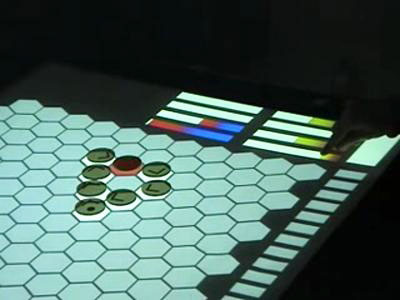
\includegraphics[scale=0.4]{1.jpg}\\
\textbf{The ReacTogon}
\end{center}

\subsection{Project Description}
Our project, branded \textit{`HEX’}, aims to emulate and extend the ReacTogon concept. Through the production of a software system that implements the harmonic table within the framework of a pattern based sequencer, we aim to provide a completely novel musical experience.\\
\\
To this end, we have written a Java application that implements the harmonic table in this way. Control is provided through the use of five counters or 'operator tiles' that are placed onto the grid, namely Play, Stop, Change direction, Explode and Warp. The latter four have active and inactive states that dictate whether they play a note or not during an interaction. In addition to this, there are buttons and sliders to change tempo and instrument. There are also multiple layers of grids, set out in tabs, for the creation of harmony and a multi textured, polyphonic composition.\\
\\
Our software is designed with a PC and touch screen in mind, as the tactile nature of interaction greatly lends itself to the interface. This said, the application will still run with a standard mouse and indeed, the nature of a Java application allows portability and support for other operating systems.

\pagebreak
\section{Background Information and Research}
\subsection{Existing Systems}
\subsubsection{Examples of Existing Software Systems}
\begin{enumerate}
\item \textbf{JR Hexatone Pro}
\begin{center}
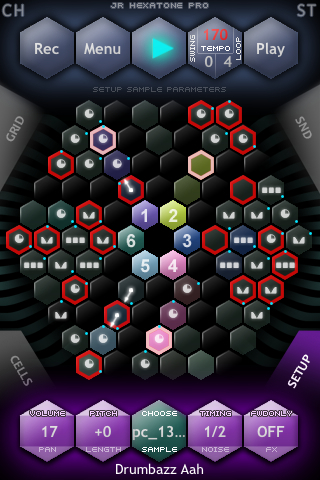
\includegraphics[scale=0.35]{2.jpg}
\textbf{The Hexatone Pro;\\ the main board of which is a harmonic table.}
\end{center}
The JR Hexatone Pro is an application developed by Amidio for iOS that implements the harmonic table \cite{jrhexitunes}.  In a similar manner to the ReacTogon, tiles or 'cell commands' are placed on a circular grid of hexagons and control the nature of the sound produced. It’s unique selling point is derived from the fact that it uses \textit{'artificial intelligence and advanced randomisation algorithms'} \cite{randomalg} to randomly alter the sound as the loop progresses to create a constantly changing sound. In addition to this, in place of a 'start' tile, sound is propagated from six 'oscillator' tiles at the centre of the grid and the playhead moves to one of three adjacent tiles. \cite{amidiomanual}

\item \textbf{TonePad / TonePad Pro}\\
The TonePad is another application for the iOS platform, developed by LoftLab.\cite{tonepaditunes} \\
\\
While it does not implement the harmonic table, it is based on a 16x16 matrix of notes in a pentatonic scale. To this end, it has a similar musical effect to notes played on a harmonic table. While the TonePad is simply controlled by selecting notes on the grid and has no placeable operation tiles, the ideas of playhead propagation and chain reactions are exemplified in this application. The playhead moves left to right across the grid and when a selected cell in the grid is encountered, it triggers others within a certain radius. \\
\\
A key feature of the TonePad application is it's ability to import and export songs. Tracks can be exported as ringtones on iPhones or to m4r files. It is also possible to export song 'code' for sharing with others; this is integrated into the app with an 'upload' button. 
\end{enumerate}

\subsubsection{Examples of Existing Hardware Systems}
\begin{enumerate}
\item Tenori-On
\begin{center}
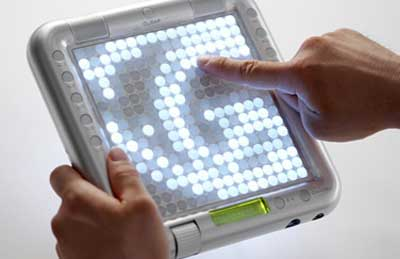
\includegraphics[scale=0.5]{3.jpg}\
\end{center}
Developed in 2005 by Japanese artist Toshio Iwai and Yu Nishibori at Yamaha \cite{tenorionwiki}, the Tenori-On is a hand-held music sequencer. Fundamentally, it is conceptually similar to the TonePad, but in hardware form and with a variety of different modes. The hardware itself consists of a 16 x 16 matrix of pressable buttons which light when activated. These buttons can act in a similar manner to the cells in the TonePad in the main sequencing mode, where highlighted cells are played when the playhead encounters them.\\
\\
In addition to this, five other modes exist such as 'push mode', which produces a continuous sound when a cell is pressed; 'bounce mode' which causes a the playhead to oscillate between the selected cell and the edge of the matrix, producing sound when 'bouncing' off the side and 'grouping' which is used to sequence patterns together.\\
\\
Each loop is composed within a layer and each layer can be thought of as 'performance parts' of which there can be a total of sixteen. Different notes and instruments can be assigned to each layer and all layers can be played together in synchronisation. Each set of sixteen layers is called a block; a total of sixteen blocks can be stored and dynamically switched between during a performance. In this way, musical loops and motifs can be generated and played sequentially to create a complete piece of music \cite{tenorionyamaha}.

\item \textbf{AXiS-64}
The AXiS-64 is possibly the most prevalent MIDI controller and piece of hardware that utilises the harmonic table. The equipment consists of the a harmonic keyboard, composed of 192 hexagonal keys; 8 preset keys for storage of user defined keyboard configurations; 4 cursor keys, for navigating between banks; a pitch bend wheel; a modulation wheel and two rotary dials \cite{cthru}. The four analogue controllers can be easily reprogrammed and used for any MIDI controller change.
\begin{center}
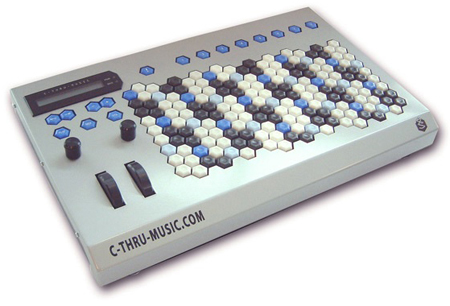
\includegraphics[scale=0.5]{4.jpg}
\end{center}
The fourth revision of the AXiS-64 firmware introduced three different keyboard modes; 'single', 'split' and 'layer'.  In 'split' mode the keyboard is split into three 64 note keyboards; in layer it becomes one keyboard sending a signal on up to three MIDI channels when a note is played and in 'single' it acts as a single keyboard.
\end{enumerate}
\subsection{Systems Research Evaluation}
The products listed above are but a few among the systems available on the market, but each one exhibits interesting or unique characteristics that can be taken as inspiration for our project. In addition to this, there are persistent themes among all products that too will influence our designs.\\
\\
Among these common themes is the use of physical interaction as an interface between the system and the user. A considerable majority of the software systems available are for tablets or mobile devices using touch screen interfaces, with almost no standard desktop applications and only a few online hardware simulations or alternatives. This information justifies our choice of using a touch screen interface with our software. In addition to this, most products act, in some propensity, as a single touch harmonic table keyboard. As such, this is an important feature to implement.\\
\\
In addition to this, particularly interesting features of researched products that we may wish to take forward into our project include the multiple 'layers' featured in the Tenori-On and the TonePad Pro's ability to export and share music and created projects. 

\pagebreak
\subsection{Market Research}
We conducted a survey (attached in appendices) targeting general music enthusiasts as well as complete beginners in the music field to find out whether our software would be desirable. Very few of the people we asked had heard of the ReacTogon, the concept instrument, but most had some sort of interactive music experience where you would either use a mouse for a desktop application or a touch screen app to create some sort of music. We received contrasting opinions on the pre-existing systems, some of them liked the idea of the program being a portable touch screen app so they can continue working on their music on the go but they also pointed out that some of the features were not as advanced as the desktop applications. The desktop applications that were reviewed were not targeted at beginner users as some of the features were too complicated and functionality was not as easy as the touch screen applications. The suggestion of a desktop application with touch screen capabilities was received well. Most said they would be interested in using a program which combined the desirable features of both a touch screen and desktop applications.
 
\subsection{Music Research}
\begin{center}
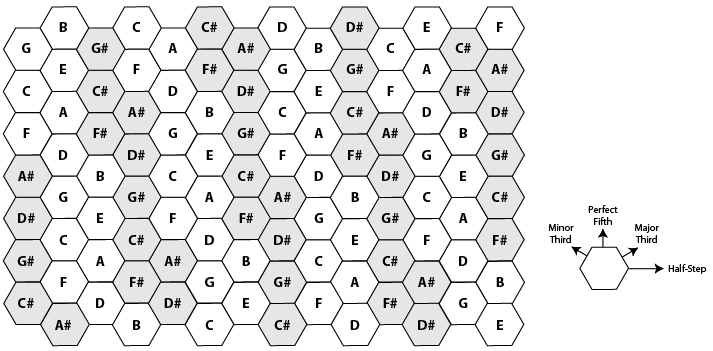
\includegraphics[scale=0.5]{5.png}
\end{center}
In musical theory, an interval is the distance between two notes or pitches, the degree of highness or lowness of a note --- based on it's frequency. Typically, these are represented with tones and semitones, where tones are the base unit of an interval. Certain intervals appear particularly often within music composition as they can provide key melodies. Such intervals include the perfect fifth, and major and minor thirds. These intervals, which are 7, 4 and 3 semitones above the base note respectively, make up the notes used in major and minor triads and are the intervals used in the harmonic table based on the following set of rules:\\
\\
\begin{itemize}
\item Notes ascend by an interval of a fifth on the vertical axis.
\item Notes ascend by an interval of a major third on one diagonal axis (north easterly).
\item Notes ascend by an interval of a minor third on the other diagonal axis (north westerly).
\end{itemize}
This layout clusters complementary notes together, for example, all the notes in the C Major chord, namely C, E and G are adjoining. Scales are played by using simple, repeated patterns that can be transposed for playing in different keys. \\
\\
Transposition, \textit{the shifting of a melody, a harmonic progression or entire musical piece to another key, while maintaining the same tone structure} \cite{koch}, 
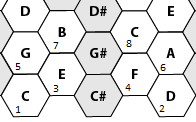
\includegraphics[scale=0.7]{scale.png}
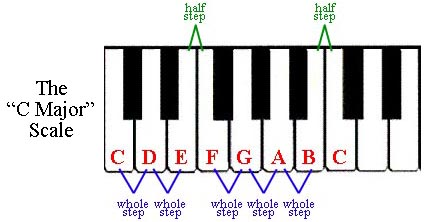
\includegraphics[scale=1.5]{scale2.jpg}
\end{center}
Above is shown a comparison of the C major scale played on a harmonic table based keyboard (left) and on a conventional piano keyboard (right). The progression is enumerated from 1 to 8.\\
\\
Scales and triads can be transposed far more easily on a harmonic keyboard than on a conventional keyboard as the basic pattern is always retained. This is shown in the G major scale below:
\begin{center}
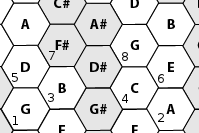
\includegraphics[scale=0.5]{scale3.png}
\end{center}

\subsection{Technical Research}
\subsubsection{MIDI}
MIDI, short for Musical Instrument Digital Interface is a technical standard that describes a protocol, digital interface and connectors and allows a wide variety of electronic musical instruments, computers and other related devices to connect and communicate with one another. (Swift, 1997). A link in MIDI can handle 16 channels of information.\\
\\
MIDI uses messages containing instruction which controls a device. A MIDI message consists of a status byte, which indicates the type of the message, followed by up to two data bytes that contain the parameters (Brewster, 2003). Using MIDI can you send ‘channel messages’ which are heard only by the channel they are sent to, or ‘system messages’ which are heard by all devices on all channels.\\
\\
Messages send data in real time over a single channel. Examples include\cite{Huber}:
\begin{itemize}
\item Note on messages: Specify a notes, volume (velocity), note, pitch and the channel it should be played on.
\item Note off messages: Same of note on, but turns off a note.
\item Control change messages: Changes instrument settings.
\end{itemize}
From this research we were able to get a full grasp of MIDI and learned that we could set each grid layer to be a channel, and each hexagon cell in the grid could send MIDI messages specifying “note-on”, with the note number, "velocity" "program" change (instrument)” and “note-off” messages. One slight disappointment we found when researching MIDI was (at the time of the research) android devices did not fully support MIDI. 

\subsubsection{Hash Maps}
Hash map is a data structure that uses a hash function to map identifying values using a key. A key is made using a hash function that will index directly into the correct position, where the correct value will be found\cite{hashm}.\\
\\
Ideally, the hash function should assign each possible key to a unique location; we will take advantage of this feature to make sure no duplicate values pulses occupy the same space in the grid.\\
\\
Because we will not be taking advantage of any algorithms to deal with collision resolution, such as Separate chaining or Open addressing the access time of the hash map will always be constant. Giving insert, search and delete a O(1) access time (Stein, 2001), which is very fast. Of course we will need an array to keep track of the keys in use.\\
\\
To create the perfect hash function we will have to make sure there are no unwanted collisions, some sort of hashing function in base 6 will probably need to be use due to the fact that hexagons are 6 sided are in a grid. \\

\subsubsection{Working With Hexagons}
The immediate area of research, on beginning coding was how to generate and work with a grid of hexagons. There are few operations one might need to perform: finding hexagon's position by its index in the grid; picking a hexagon by mouse; finding neighbour cells; finding hexagon's corner coordinates etc.\\

\begin{center}
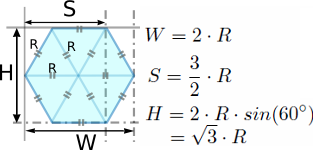
\includegraphics[scale=1]{diag1.png}\\
\end{center}

Using simple properties of hexagons, as shown in \textit{Fig. 1}, we are able to derive useful methods of manipulating and arranging them, and produce relevant algorithms for use in our code. \\
\\
We define the hexagon by its radius R, and find some other parameters based on it, such as W ("width"), S ("side") and H ("height"). We can calculate W,S,H easily with a known R.\\
\\
Hexagon grids can be derived from square grids. Since coordinate systems for squares are much easier, the derivation will guide us in designing coordinate systems for hexagons\cite{grids}. To turn a square grid into a hexagon grid, there are two steps needed. First, we must offset the columns (or rows). Second, we should split half the square edges and bend them in the middle.
\begin{center}
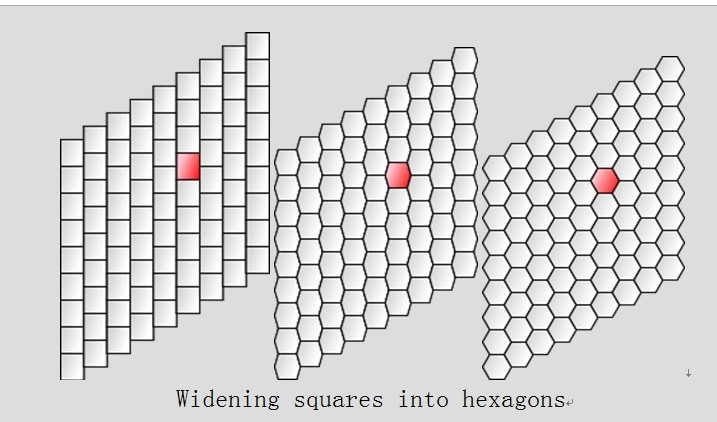
\includegraphics[scale=0.5]{image11.jpg}\\
\end{center}
The most common way \cite{gdmath} to offset columns is to offset every other column. Code using this approach looks at whether it is an odd or even column and chooses whether to offset it. A simpler approach is to offset each column by half a height more than the previous column. Code using this approach is more uniform, but the map shape is no longer rectangular, which can be inconvenient.\\
\\
With either offset approach, the next step is to split the vertical edges of the squares and bend them. When the bend is reduced from 180 degrees to 120 degrees, we get regular hexagons.
\subsubsection{Identifying Hexagons}
\begin{center}
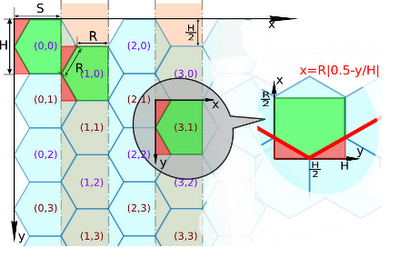
\includegraphics[scale=0.5]{image10.png}\\
\end{center}
From the picture above, we can figure out the formula for finding position of the top left corner of a hexagon cell by its array index (i, j):\\
\begin{center}
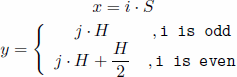
\includegraphics[scale=0.5]{image16.png}\\
\end{center}
With this knowledge we are now able to perform basic the operations and manipulations with hexagons necessary for use in our software.
\section{Requirements Specification}
Our project has several important key features which need to be followed and implemented; they can be described in the functional, in other words, definitions of what the system must do; and non-functional requirements, definitions of how the system is supposed to be. These are detailed henceforth:
\subsection{Functional Requirements}
\begin{enumerate}

\item The application must be able to play a note at the press of a hexagonal tile on the grid.
\begin{enumerate}
\item It must be possible to manipulate the sound through variation of voice/MIDI instrument.
\end{enumerate}

\item The application must implement the Harmonic Table in the layout of playable notes.
\begin{enumerate}
\item The notes must be set out on a grid of contiguous hexagons.
\item Moving immediately up a hexagon will increase the pitch by an interval of a 5th and vice versa.
\item Moving immediately right a hexagon will increase the pitch by a semitone and vice versa.
\end{enumerate}

\item `Operator tiles' should be placed on individual hexagons within the grid to manipulate sound in various ways.

\item The following operator tiles should be implemented:
\begin{enumerate}
\item \textit{Play} - Begins the sequencer, sending an initial pulse in a straight line in a specified direction.
\item \textit{Stop} - Stops and `absorbs' the pulse at that position.
\item \textit{Change} - Changes the direction of the pulse.
\item \textit{Explode} - Causes the pulse to 'split', propagating new playheads from each edge of the hexagon it is placed on, but not going back on itself.
\item \textit{Warp} - When the playhead meets a warp tile, it will spawn new playheads at each other warp tile placed on the grid, moving in the direction of entry. 
\end{enumerate}

\item Tempo must be controlled in two ways:
\begin{enumerate}
\item A global base tempo must be set.
\item Tempos on each grid can be set independently.
\begin{enumerate}
\item Individual grid tempos must be a multiple of two, relative to one another.
\end{enumerate}
\end{enumerate}

\item A moving 'pulse' or 'playhead' should be used to trigger tiles placed on hexagons.
\begin{enumerate}
\item The playhead must move faster or slower based on the tempo specified.
\item The playhead must move consistently with the tempo specified.
\end{enumerate}

\item Each operator tile should have an off or an on status, which dictates whether it will play a note when encountered by a pulse.
\begin{enumerate}
\item The sound produced is based on the position of the tile on the harmonic table grid, rather than the tile itself.
\end{enumerate}

\item Operator tiles should be removed with a delete mechanism.
\begin{enumerate}
\item When a `delete' key is depressed, a click must remove a tile from the grid.
\item There must be a `clear' button to remove all tiles from an individual grid.
\end{enumerate}

\item The following operator tiles must be able to rotate when placed in order to send the playhead in different directions:
\begin{enumerate}
\item \textit{Play}
\item \textit{Change}
\end{enumerate}

\item Six grids should be implemented for use in harmonic, polyphonic projects.
\begin{enumerate}
\item Grids must be independent.
\item Different tiles must be able to be placed on different grids.
\item Each grid must be able to have it's own tempo.
\item Grids must be able to be played simultaneously.
\end{enumerate}

\item Global `Start' and `Stop' buttons should be implemented to start and stop playheads over all grids.
\begin{enumerate}
\item Individual grids must be able to be selected and deselected for play.
\end{enumerate}

\item Saving and loading must be implemented for ease of producing and sharing projects.
\begin{enumerate}
\item Individual grids must be able to be saved independently
\item Projects must be able to be saved as a whole.
\end{enumerate}

\item The application must implement a control system suitable for a touch screen and also mouse interface.
\begin{enumerate}
\item The application must be controlled through use of single touch sliders and buttons.
\item It must have either `tap to scroll' and/or `drag and drop' selection.
\item Menus must be available through a single click mechanism.
\end{enumerate}

\item The menu must contain at least the following key features:
\begin{enumerate}
\item Create new project.
\item Save/Load.
\item Select Grid.
\item Change instrument on a certain grid.
\item Select grids to play.
\item Open help screen.
\end{enumerate}

\end{enumerate}
\subsection{Non-Functional Requirements}
Our application is aimed to be used by a wide variety of people, with varying levels of musical capability. With this in mind we must place much effort into making the application as accessible and easy to use as possible. As such, it is important that our project conforms to the following principles:

\begin{enumerate}
\item Extensibility - The application should be fully extensible, i.e. adding new features, and carry-forward of upgrades should be viable while maintaining the core mechanic.
\item Maintainability - The application should be easy to maintain.
\item Performance - The application should run comfortably on a wide range of computers.
\item Usability - the application should be easy to use and have simple, intuitive user input.
\end{enumerate}

\part{Design}
\section{Software Design}
We looked at the Reactogon and decided to expand upon it, please look at the functional requirements for this.
\subsection{The Grids}
Our software would comprise of 6 layers; each layer being a grid. Each grid would have to be unique yet have different properties; this was the first clue to using OO design. Each grid would have a set of properties, these properties being:
\begin{itemize}
\item Each grid could be assigned a unique instrument, but needs to support changing it on the go during mid play. This suggested that a grid could be assigned its own channel in a MIDI sequencer. (Rees, 2001)

\item Each grid could support different octaves, through the research we found that MIDI can play 127 different notes ranging from octaves 0 to 10, our grids therefore need to be able to be transposed mid session. This suggests that each grid have a starting note and some sort of algorithm then fills the grids with correct notes.\\
\\
The tempo of the grid should be changeable, but all grids needs to have some sort of relation to each other, so some sort of base tempo needs to be applied, then each grid can then play at $ 1 \times , \frac{1}{2}, \frac{1}{4}, \frac{1}{8}$ or $\frac{1}{16} $ times that pace, these values were chosen due to the research in music theory. This implies that a grid can be halted for set amount of time/tick.
\end{itemize}

The grid itself would be made up of hexagonal `cells’, these should hold information about what note each cell is, this could simply be a number. From this it would be sensible to store the cells as a 2D array. As discussed above this would then make it quite simple to transpose notes with an algorithm. Information about where it should be placed in the grid itself. Some of the properties of hexagons are outlined in the research and will help for placement and using hexagon properties to our advantage. Because this is quite a visual piece of software some information needs to be held about its state, as we wanted to show if a cell is active or not.

\subsection{Pulse}
The vision of a pulse is some sort of object moving through the grid, from cell to cell. The pulse itself should be quite simple as all it must do is move from one cell to another. The tempo of the grid should manipulate how fast the pulse moves from one to another. The grid must be able to support multiple pulses, all moving in different directions at the same time. As well as this, pulses must not affect one and other, crossing/colliding pulses shouldn't be a problem and the software must be able to handle this. But the software must be able to handle pulses that occupy the same space, as not to create exponential loops see figure 1. When a pulse comes into contact with a tile it should affect the pulse in some way.
\begin{center}
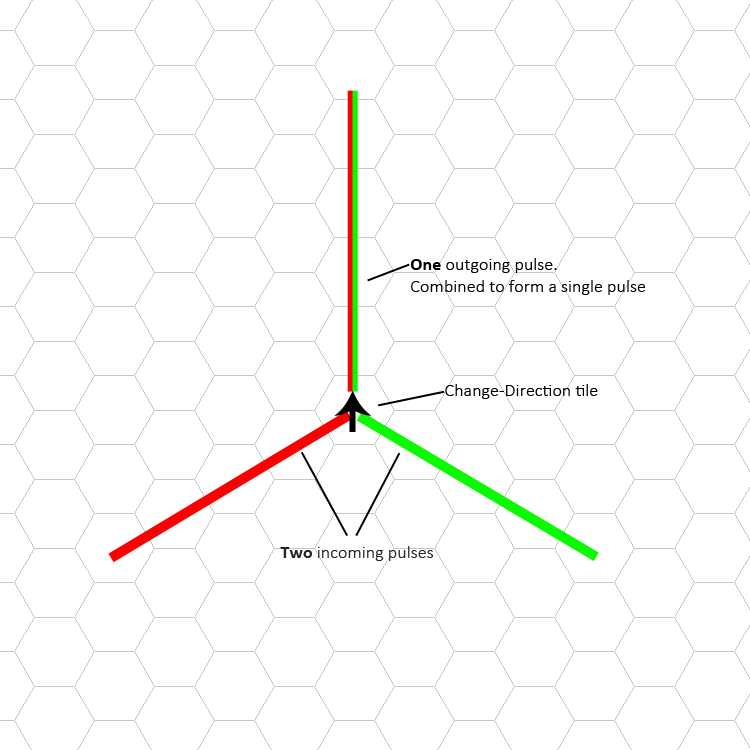
\includegraphics[scale=0.5]{6.png}
\textbf{fig. 1}
\end{center}

\subsection{Tiles}
The main idea of this software is the use of tiles to manipulate the music. A tile can be placed in a cell on the grid and used to manipulate an incoming pulse. Different tiles have different effect. The tiles are listed as follows:
\begin{itemize}
\item    Stop: Should destroy the pulse

\item Change direction: This implies that the tile should hold a direction and then be able to pass this information onto an incoming pulse. Because the tile will have different arrows for different locations will mean that the graphics will have to be redrawn with the corresponding arrow.

\item Play: Will work in much the same way as change direction as it should be able to change a pulses direction. As well as this it will be the starting position of a pulse, maybe creating it.

\item Explode: Will destroy and incoming pulse in much the same way as stop does, but in turn create 5 new ones and send them in every direction apart from the input. From this knowledge it would be sensible to assume that a pulse should hold information about its previous position in the grid.

\item Warp: Will ‘warp’ a pulse from one place to another,  if multiple warps are places then the pulse should come out of those tiles also. From this I will make a warp tile destroy a pulse, and create new ones in all output locations. There will need to be some way of storing locations of all warp tiles in a grid, all with their own unique id.
\end{itemize}

The tile object should therefore have a ‘type’ and a direction at minimum. When I pulse comes in contact with a tile it should play a note, but there are also tiles that should not play a note, this means there must be some data variables stored in each time if it should play a note or not when hit by a pulse.

\subsection{Keeping Time}
The whole system needs to be produce music at a reliable rhythm, therefore there needs to be some timer that tells each grid to increment all the pulses why one step. The timer must always have the same interval.

\subsection{Creation of Sound}
If 4 separate pulses hit 4 different tiles on the same ‘tick’, they all should be played at the exactly the same time, and all 6 grids must follow this rule. For this to happen, there needs to be some sort of queue, where all notes that should be played at a set point in time are grouped together, then sent off to be played all at once. This could happen multiple times per second, so it looks like some sort of thread will be needed to play multiple sequences at the same time and will not halt the program.

\section{User Interface Designs}
The colour scheme of our software is grey-scale, with blue and orange highlights. This is comparable to the popular video game portal 2, and allows for easy differentials to be made between different functions of each tile, as well as allowing for an attractive overall look. The design of the tiles has been through several iterations as can be seen below:
\begin{center}

\includegraphics[scale=0.5]{tileprogression.jpg}
\end{center}
In the end, we decided on a drop shadow chrome look, accented with each colour depending on the corresponding tile's purpose. The progression is from left to right, and illustrates the process in which I went through designing the tiles. We started with a functional place holder, before investing more time into the appearance of the tile for the second iteration, and finally made a high resolution version for implementation. Each area of the graphics underwent a similar design progression, as can be seen here.\\
\\
The progression of the logo design can be seen below, and illustrates a process of refinement which involved critique from group members and my own design input.\\
\\
\begin{center}
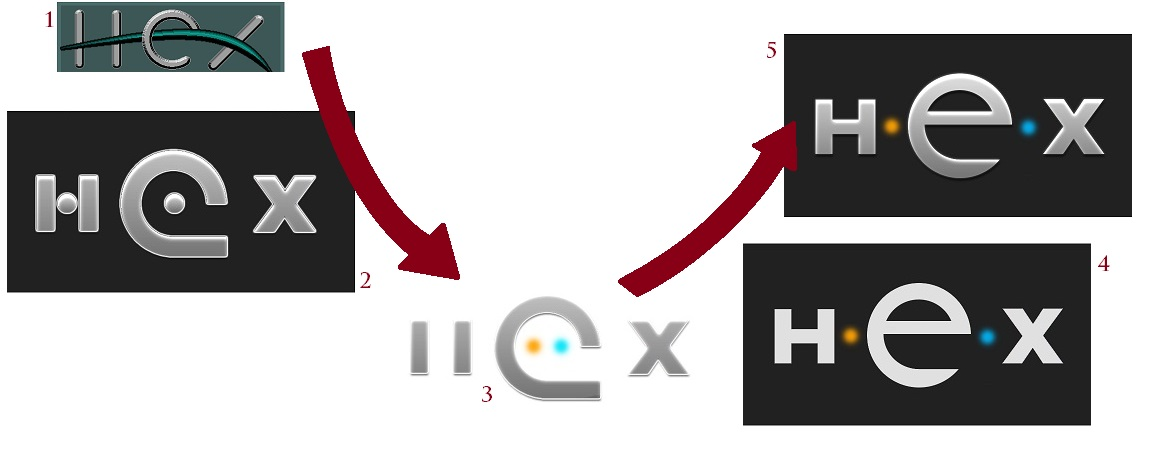
\includegraphics[scale=0.5]{logoprogression.jpg}
\end{center}
The controls section of the window changed over time, as we added new features to the project, and I developed the design theme and layout as time went on. The first version I put serious time into introduced the metallic them to compliment the logo and tiles, and although this was well received, there were a few issues with the chunkiness and curviness of some aspects. In order to improve beyond this, I took a new look at it and decided to split the window into two halves, move the tabs, and start a more simplistic controls look. This was very well received, so I polished things up and completed the design with this look, which is what our finished project looks like:
\begin{center}
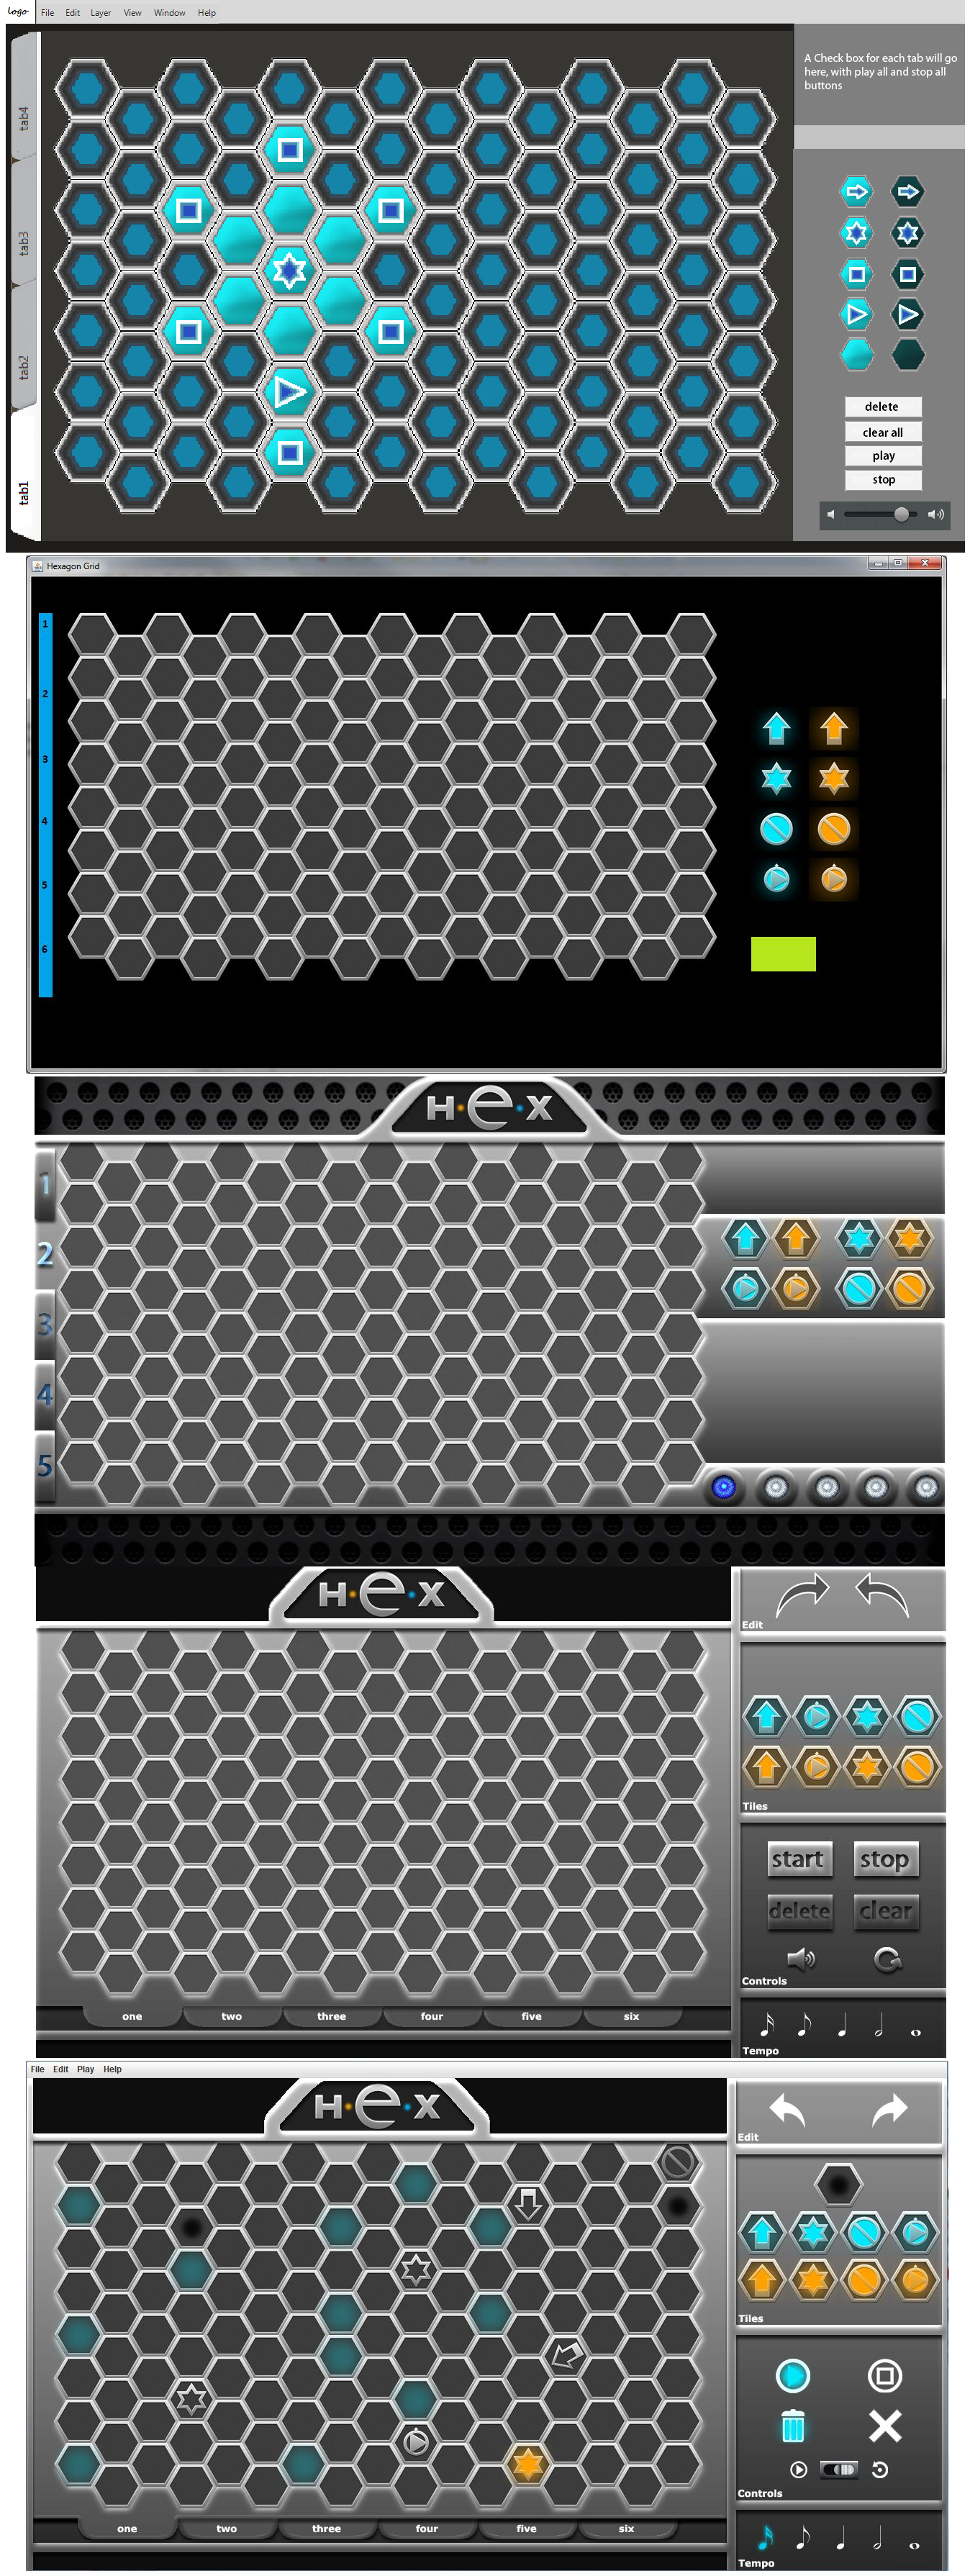
\includegraphics[scale=0.26]{controlprogression.png}
\end{center}
As you can see, we have a consistent colour scheme, with elements of each part of the static and interactive design visibly tied together to give the impression of quality and completeness.\\
\\
Below is a description of the various features of our software's layout as labelled here:\\
\\
\begin{center}
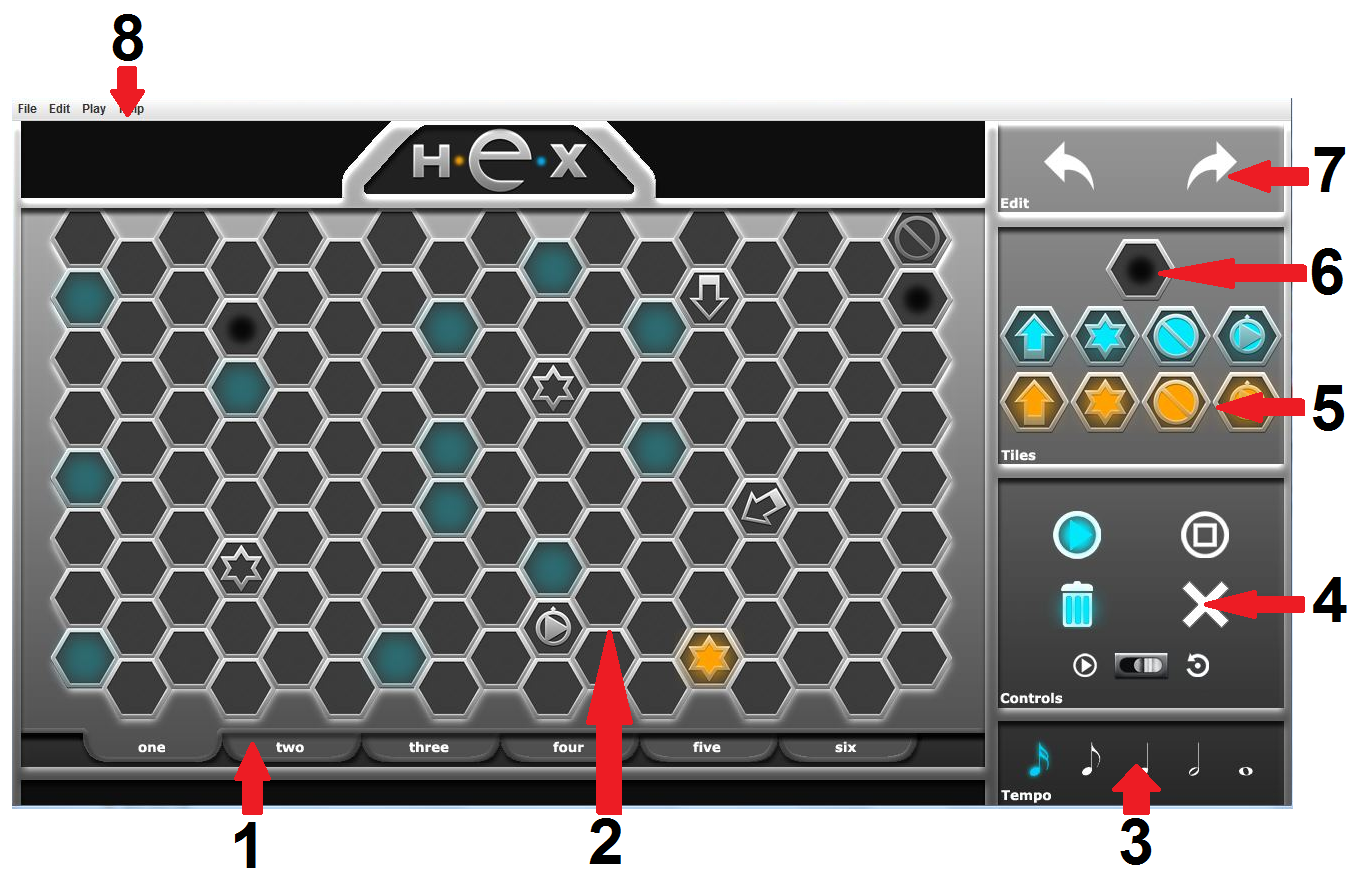
\includegraphics[scale=0.35]{numlayout.png}
\end{center}

\begin{enumerate}

\item This is where the user changes the tab they are editing. The design of this tries to make it obvious that the tabs are above one another and how to change between them.
\item The grid makes up for the bulk of the window real-estate, and rightly so as it is the main interactive element of the program. This is situated as can be seen, in the centre of the GUI, to the left of the controls.
\item The user can change the tempo of the current tab here. The symbols of semiquaver, quaver, crotchet, minim and semibreve represent 16x, 8x, 4x, 2x, 1x, from left to right, respectively. This is to allow for an intuitive control of the current tab's tempo.
\item This is the controls section of the control bar. It includes buttons which start/stop the pulses, enable deletion of individual tiles or clear the entire grid. Below these controls is a switch which changes what happens when the user clicks on the grid. The right hand selection will rotate a tile clicked on, and the left hand option will play the note corresponding with where the grid was clicked.
\item This is where the tiles are placed. The blue tiles play a note when hit by a pulse, and then carry out their function, whereas the orange tiles carry out their function silently. A user clicks on a tile before choosing where to place it in the grid.
\item This is the latest tile addition and is different to all the others. It allows the user to transport the pulse and its direction across the grid, without having to travel there. It is called the warp tile and is selected and placed like the other tiles.
\item This is the edit section of the control bar. It allows the user to undo or redo any actions on the grid. The selection of grids to be played is now located in the menu.
\item The menu bar is situated at the top left for conformity reasons. On a windows application, the menu is regularly here, and this is what our software is designed for.

\end{enumerate}

\part{Implementation}
\section{Key Control Elements, Data Structures and Methods}
\subsection{Removal of Duplicates}
Removal of duplicates, figure 1 in the design shows a problem of pulses merging together. Two or more pulses could occupy the same space and this would cause the amount of pulses to exponentially grow and in turn cause the program to slow down and eventually crash.\\
\\
This was due to pulses being held in an array, to removing duplicates from this array would take $ O(n^{2}) $ time, and even then it would still have problems detecting them. To solve this problem, a hash map was used to store the location of the pulse in the grid. The hashing algorithm took the pulses current location, and direction to place it in the hash map, the hashing algorithm is shown in below (equation 1). The hashing algorithm was relatively simple because by virtue of using hexagons it was possible to work in base 6. By doing this, if two pulses occupied the same space on the gird (going the same direction etc.) they would be placed in the same position in the hash table; this would cause a collision, but as a hash table only accepts unique values, the second value (and any after that) would simply write over the old value. See the Hash Maps section of Technical Research for more.\\
\\
To keep track of the keys in the hash map there is an array list holding all the keys that are currently in use, to access the pulses it was necessary to traverse through this list and use the keys to get data from the hash map. Every loop, the array list was emptied and all keys where added again. By using a hash map access time was reduced to $O(1)$ and removal was never a problem, as a hash map with no linear probing just writes over a value. It also meant I was not adding and removing lots of pulses from an array list all the time.\\
\begin{equation}
Key = ((Pulse.tLocation \times 36) + (Pulse.fLocation \times 6) + direction)
\end{equation}

\subsection{Timing and Tempo}
Timing the whole system was very important. To do this I used Timer that was scheduled at a fixed rate. This meant that it would call the run method every set amount of time irrespectively if it had finished the methods or not. The timer controlled how often the pulses moved one space in the grid. Because each grid could have a different tempo I needed to keep all the grids synchronised but still have different tempos. To do this in grid a tempo is assigned with a value of 1, 2, 4, 8, or 16.\\
\\
Then every loop of the base timer a value is incremented by 1 this value is then MODed against the tempo of each grid, if it is 0 then it will move the pulses inside this grid by one, it if it not it will skip this grid. This is explained clearly in the below code for the \textit{play()} method. At the end of every loop queues of notes are played, this keeps everything in sync.\\
\begin{center}
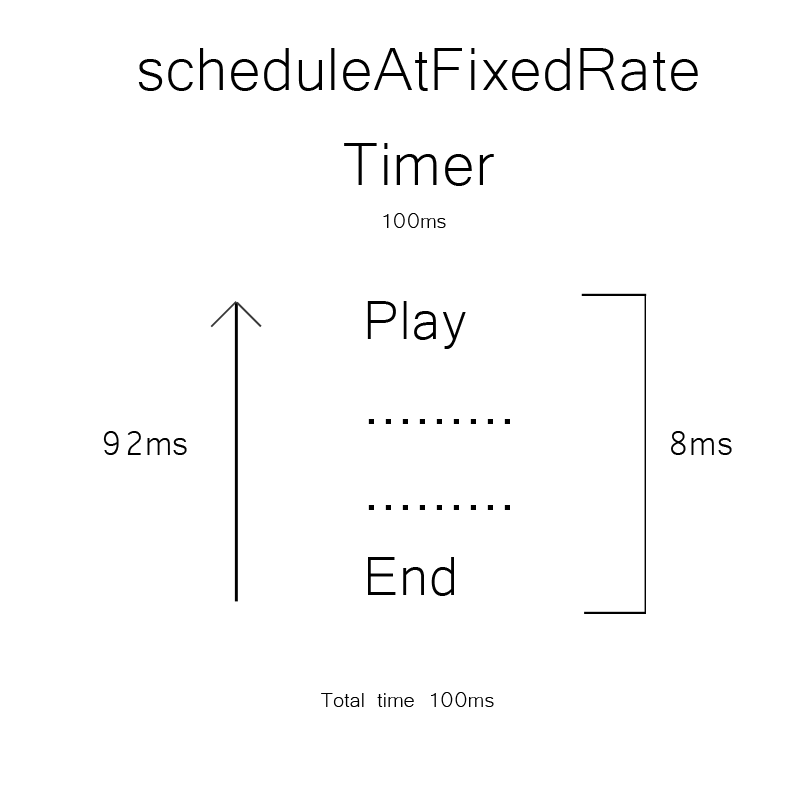
\includegraphics[scale=0.2]{utimer.png}
\end{center}
\subsubsection{\textit{play()} method Implementation}
\begin{center}
\begin{verbatim}

function play() 
    if (tempoControl > 16) 
        tempoControl = 1 
    for all grids 
        if (tempoControl % grid.getTempo == 0) 
            grid.play() 
    tempoControl++
    playNotes() 
	
\end{verbatim}
\end{center}

\subsection{Transposition}
\begin{center}
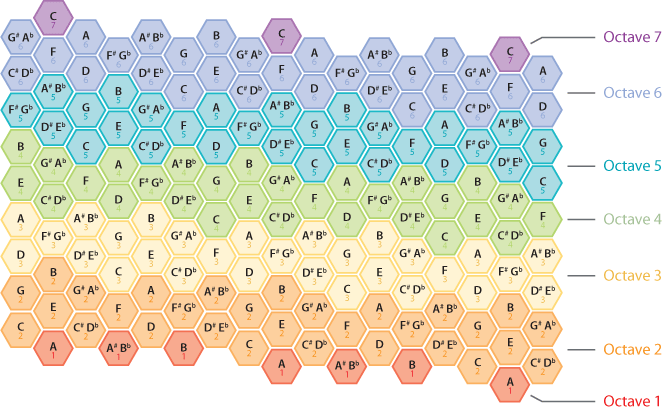
\includegraphics[scale=0.5]{7.png}
\end{center}
One feature of the program that was much easier to implement than expected was being able to transpose the whole grid and changing the start note of each grid on the fly. You could use the fact hexagons where stored in a 2nd to your advantage and that MIDI notes could be stored as numbers. Studying how the harmonic table works (above), and finding patterns how the notes were placed we were able to write a simple formula (below), that selecting a start node of the grid, it could then place the correct notes in the correct place. Putting this formula then in a loop that goes through the array meant it could be called at any time even during play, as hexagon cells themselves held the note numbers. This formula would work for any size grid, so if we wanted to extend the table at some point that would be possible. \\

\subsubsection{Transposition Formula}
\begin{center}
\textit{The note for any given i, and j cell on the grid can be given by:}\\
$ n = startNote - (7 \times j) \linebreak note = ((n + 4) - ((( i \% 2) \times 7))) $
\end{center}

\subsection{Sound Production}
The sound creation went through many stages, and indeed, could still be seen as a work in progress. The most important of the system was keeping everything synchronised. If 20 notes were scheduled to play at the same time, then they all should be played at exactly the same time, not milliseconds apart. To do this you can see in figure 3 there is a method call playNotes() this would play a track containing all that notes that had to be played at that moment in time. The way the notes were added to this track was; As you now know, the pulse move through the grid, step by step, if it came into contact with a tile it would have an effect. If that tiles properties were set for it to play a note, then a method was called (figure 8), and the note for that hexagon was passed into the sound sequencer, each note had an on, off and instrument set to it. Once one whole loop had gone through, the playNotes() method would send this track off to a sequencer in a new thread and play them all at once, this would happen repeatedly every loop. Figure 9 explains this in picture form. 

\begin{center}

$ soundSequencer.queueNote(hexCellCurrent.getNote(), channel);  $\\

\textbf{queueNote Method}
\medskip 
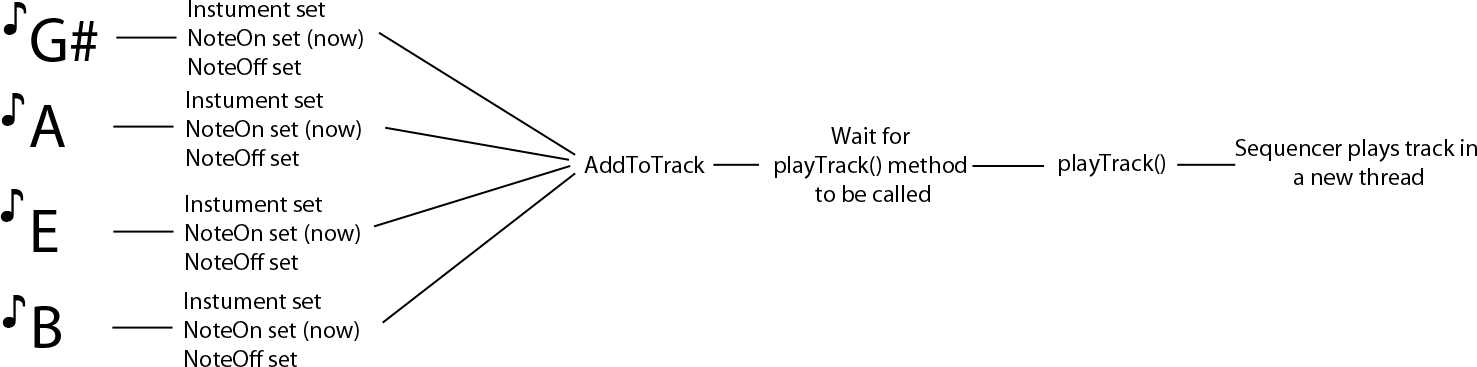
\includegraphics[scale=0.25]{8.png}
\end{center}

\pagebreak
\section{Code Plan}
\begin{center}
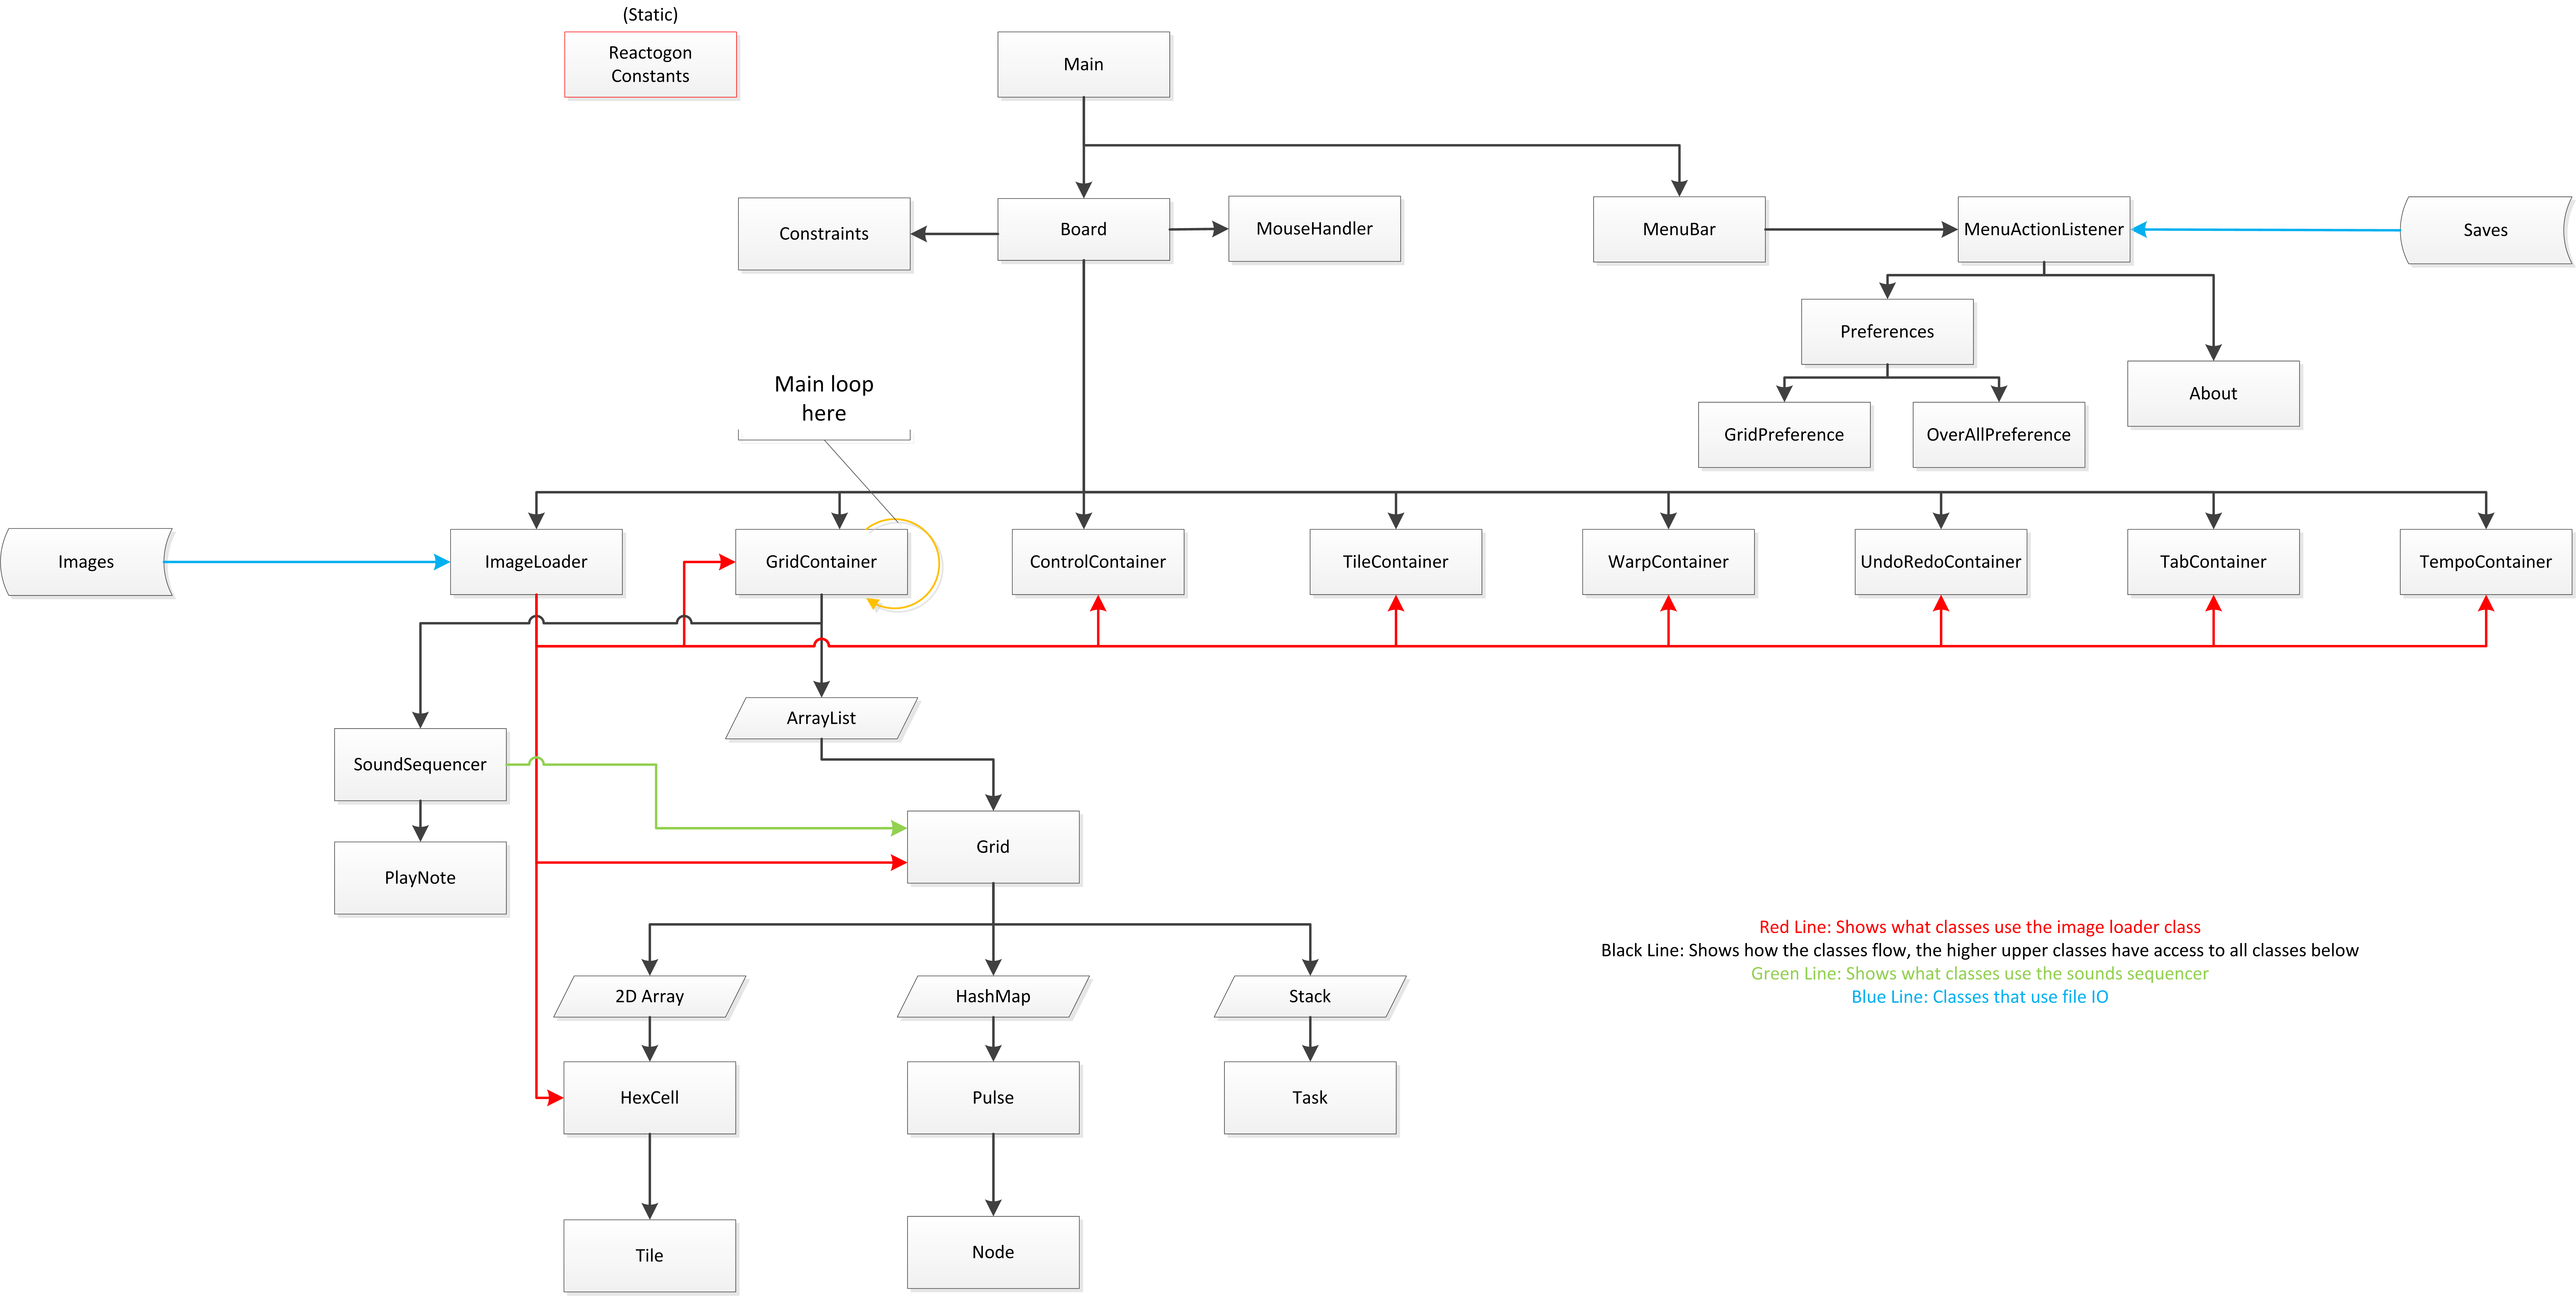
\includegraphics[scale=0.65, angle=270]{plan.png}
\end{center}
\pagebreak

\section{Testing}
\begin{center}
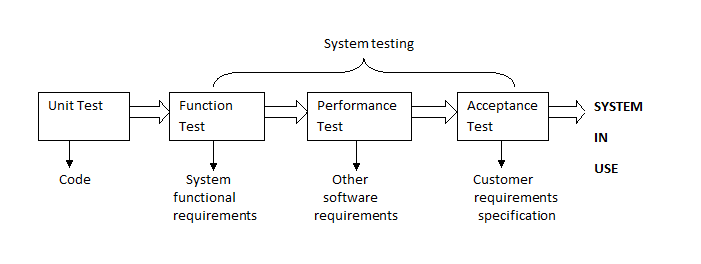
\includegraphics[scale=0.5]{9.png}\\
\textbf{Planned Testing Phases}\\
\end{center}
The objective of testing is to find faults, defects in design, requirements and in code\cite{SEP}. With the help of testing, the defects would be fixed and the program can be improved to better meet customer’s needs. In addition, if tests find few faults, it can give confidence in the quality of our software. Our tests are planned to be completed in 4 phases which is unit test, function test, performance test and acceptance test. Once some components of our program are coded, we begin to test. This part only provides a discussion on the testing of the system, the detail test cases are given in Appendix 3. 
\subsection{Unit Testing}
Unit tests are written with JUnit. Some codes are written to provide a predetermined set of data to the components which are being tested and observe the results and check the internal data, logic, boundary conditions for input and output data \cite{SEP}. To write unit test, the first step is to read through the code and figure out what exactly the functions, the classes do. Make sure the code can be compiled and use some example data as input and compare the output with the expectation result. In JUnit, the function assertEquals() is usually used.\\
\\
For example, the class HexCell create a hexagon, calculates dimension, note and image of it. There are some functions like getImage(),flipState(),setNote() etc in it.\\
\\
A class HexCellTest is created as a unit test. In this test class, some initial values are set up.\\
\\
Example code: $ assertEquals(il.getImage(tile, state), hc.getImage()); $\\
\\
The code above is to test method getImage(). The first parameter in assertEquals() is the expected output and the second one is the actual output, if they are the same, when running the JUnit, the test of this method can pass which means the components which are being tested meet the requirement.\\
\\
There are other unit tests like PulseTest, TileTest. Some example data is provided to test the methods. Other test codes are provided in the project file.\\
\\
When finished testing the code, the system testing can be initiated. 

\subsection{Functional Testing}
Function tests are run to check whether the program is satisfying the customers' needs, they are based on the functional requirements. Our functional tests work at two levels:
\begin{enumerate}
\item Code level: Add System.out.println() in the code to print some example output data and check if it is processing right.\\
For example, code ‘System.out.println("Note ="+note); ‘ is added in method playNote() and queueNote() to show the MIDI note numbers.
\item  User interface level. Observe the results in the user interface level. For example, observe the image, the light and the sound which the application actually presents. Compare these with the result that the users are expecting. If they are exactly the same, the test is passed which means it meets the requirement. Otherwise, the test is failed and debugging is needed to make the test pass. An example test is shown below:
\end{enumerate}

\subsubsection{User Interface Testing Example}

Functional requirement to test: Explode operator tile which can split a pulse into 5 different directions should be implemented.\\

\textbf{Test steps:}
\begin{enumerate}
\item Click and place the blue ‘play’ button on the first hexagon tile.

\item Click and place the blue ‘explode’ button on the second hexagon tile which is in the direction of the first one.

\item Click ‘start’ button.
\end{enumerate}

\textbf{Expected result in steps:}
\begin{enumerate}
\item Should display a grey 'play' tile on the first hexagonal tile

\item Should display a grey 'explode' button on the second hexagonal tile

\item Should play a note and display blue light which represents the pulse from the first tile to the second tile. Then should play a different note at the second tile and display blue lights from the second tile to all directions except the opposite direction of the first tiles.
\end{enumerate}

\textbf{Actual result in steps:}
\begin{enumerate}
\item A grey “play” tile displays on the first hexagonal tile. Example output data: The node is (10,6)

\item A grey “explode” tile displays on the second hexagonal tile. Example output data: The node is (10,3)

\item The application plays a note and a blue light displays from the first tile to the second tile. Then the application plays a different note at the second tile and display blue lights from the second tile to all directions except the opposite direction of the first tiles’.
\end{enumerate}

\textbf{Example output data:} $ Note =67. The direction is 0. The node is (10,6). Now the direction is 0. The node is (10,5) $ …

This output data is very long and the complete data is shown in the appendix. The actual results and the accepted ones are the same after comparing. Hence this test is passed. There are be a quite a lot of functional testing to make sure that the system operates as required and the detailed test cases are provided in appendix 3. 

\subsection{Performance Testing}
Performance tests are run to check whether the program meet the nonfunctional requirements. We decide to cover three types of performance test which are stress test, compatibility test and usability test. 
\subsubsection{Stress Testing}
This test is to ensure the software does not crash in conditions of insufficient computational resources such as low memory or running out of disk space.\\
\\
The CPU utilization rate is used in this test, although this test may not be very accurate for the reason that the CPU usage rate is always changing in a small rage.\\
\\
\textbf{Test:}
Before run the application, the CPU usage rate is 0~1. When open the application it rise to 38 at most and stabilized around 8. When put the operator tiles on the grid and start to play note, the CPU usage rate is around 7 to 12. There is no obvious changes when increase the number of tiles on the grid. When use more grids to play note concurrently, the CPU usage rate increase to around 22 at most and stabilized around 9. The average CPU utilization rate of the application is around 5.7. Hence, our application’s CPU usage is not very high and it is not easy to crash even in conditions of insufficient computational resources. 

\subsubsection{Compatability Testing}
The compatibility testing is based on the non-functional requirement that the application should run comfortably on a wide range of computers. It is done to check if our application can run on different configurations of hardware. The application is tested to run on my laptop at home, my classmate’s computer, computers in school lab and library computer. It can run successfully on all. Other tests have been run on various linux distributions and have all been successful. Therefore it can be concluded that the application does run on Windows 7 and the sampled linux distributions.\\

\subsubsection{Usability Testing}
Usability testing, which is also called human factors testing, is based on the non-functional requirement that the application should be easy to use. It is concerned mainly with the use of the application.\\
\\
The test is divided into two aspects. The first one is to test the efficiency of using the application, calculate the time and the steps to complete basic tasks such as load a hex file, save a hex file and stop a beat. The application can respond immediately to complete tasks. And the steps are designed to be minimized. When start runs the application, the time to create layout is 505.0 ms(in some computers, the time may be longer).When using the application, for example, to play note through operator tiles, the basic steps are clicking the operator tile you want to add, clicking on the place on the grid and finally clicking the “start” button. And it only cost several seconds.\\
\\
The second one is to test the emotional response. It is to check if the user interface is easy to use and understand. Our application contains a clear background, clear layout and meaningful images for the control buttons. There are few words on the board to make things simpler. When the user does not know the meaning of the icons, the help menu can be used. In addition, the users may make mistakes and the edit button ‘undo’, ‘redo’ can be useful. Furthermore, Keyboard Shortcuts are enable to make sure the ease of use. The customers’ feelings are asked in the acceptable test. 

\subsubsection{Acceptance Testing}
The acceptable tests are conducted, evaluated by users. So we ask some other people to use our application, ask them to check if our application can meet their needs. This can also test the installation of the software when we run the software on the other computers. This is an ongoing test with each release of our software.

\part{Project Meta-Comment}
\section{Updates since Interim Report}
There have been numerous updates to the project as a whole since the last report. The most obvious change is the overhaul to the software frontend and graphical user interface. Placeholder graphics have been replaced with finalised, heavily improved designs for a more immersive and polished feel, this is described in detail in the User Interface Designs section. In addition to this, a menu system has been added, where most major functionality can be accessed. \\
\\
In terms of changes to functionality of the software, since the interim report we have implemented multiple grids; the \textit{Warp} tile; the ability to change grid tempo and instrument on the fly and saving and loading have been finished and added.\\
\\
The code has also been vastly improved in terms of efficiency, having completely rewritten the sound sequencer, decreasing memory usage and required CPU time.\\
\\
Overall, in terms of improvements and updates, we have attempted to turn what was effectively a prototype into a finished, complete product.\\
\section{Time and Planning}
At the start of the project we immediately contacted each other via email to meet in order to organise meeting times and to assign roles within the project to each team member. After comparing each other's timetables we agreed to meet 4 times in a week; one 30 minute formal meeting with our supervisor, one 1 hour informal meeting at the beginning of each week to separate tasks for that week and review tasks completed the previous weeks, a 4 hour group working session and a quick 20 minute meeting before our formal meeting with our supervisor. We also agreed early on that the best way to monitor our progress and organise our time would be to create a Gantt chart (See below). \\
\\
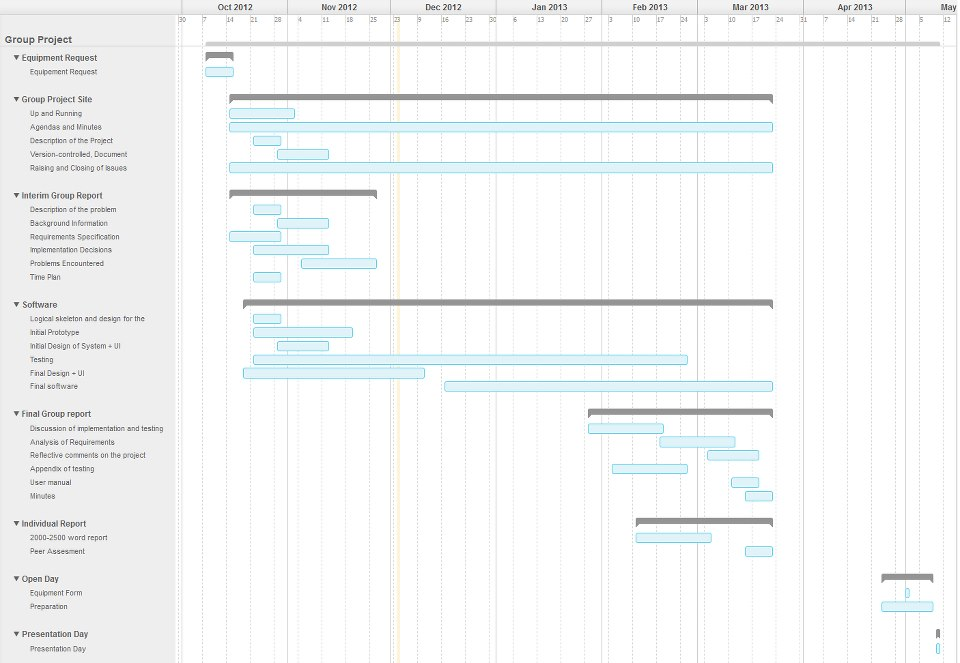
\includegraphics[scale=0.7, angle=270]{gantt.png}
\pagebreak
The first thing we needed to do was create work breakdown structure so we separated tasks into different topics and then created sub-topics for each. Using deadline dates as guidance we made a rough estimate of how long each task will take then broke that down further for each sub topic and finally determined the order of the tasks. There is also a percentage complete column inserted, which was updated regularly so we can view progress on that particular section. We can also see if we are on track to complete each section. Using the Gantt chart we could view the critical path of the project as a whole. Critical path analysis shows an overview of the time-scale of the project - showing us if we are on track to complete the project on time. The critical path allows for slack time, so if a task is taking longer than necessary then it can be compensated as tasks overlap and eventually the critical path is not affected. For each subtopic, tasks were created and placed onto an online Kanban board.\\
\\
\begin{center}
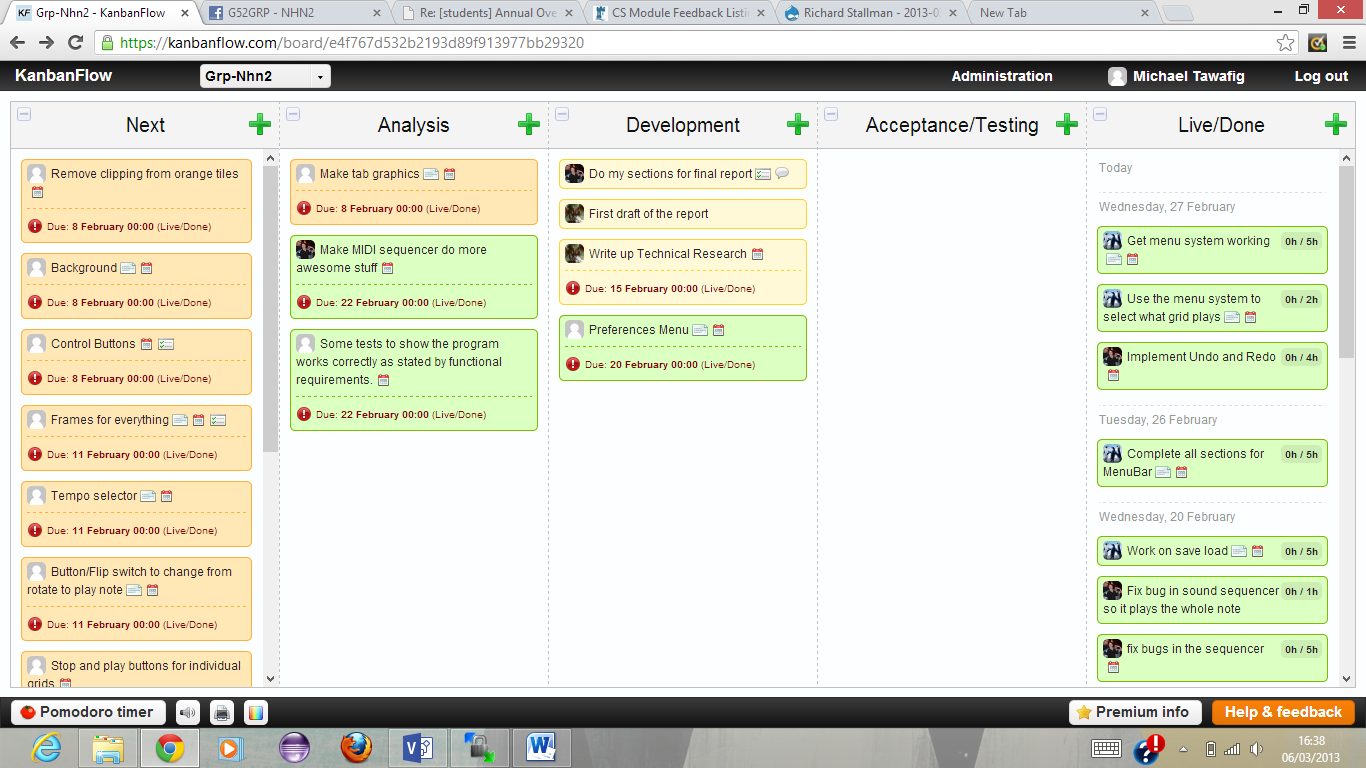
\includegraphics[scale=0.3]{kb.png}
\textbf{KanBanFlow Main Board}
\end{center}
In our 1 hour informal meetings we were all assigned tasks for that week; these tasks were placed on a Kanban board using \cite{kb}. A Kanban board is an electronic board, which contains all the tasks in the product backlog (tasks that need to be completed); each task is separated into different columns, tasks that need to be done, tasks being analysed, tasks in development, tasks being tested or awaiting feedback and finally tasks completed. Each task has a name and description, each type of task is colour coded to correspond to a topic in the Gantt chart and also is an effective way of differentiating between the types of tasks. A team member is assigned to each task and a time estimate is made, when a task is completed the team member responsible fills in the time it took them to complete it. While a task is being done each member can show their progress by moving their task to the appropriate column. Each task has a due date and as it is an interactive board, it sends reminders to your email to tell you a task is due soon. The Kanban board was a very effective way of assigning tasks to each other and also a brilliant overview of the immediate tasks that needed to be completed. By using the Kanban board we were able to create a pert chart using the tasks.\\
\\
 A pert chart is similar to a Gantt chart but for a shorter timescale and each task in it is more detailed and specific. By using the tasks on the kanban board, we created a weekly Pert Chart to ensure the weekly tasks were completed and if any task is taking longer than usual then we were able to compensate as a critical path was determined first. As tasks weren’t completed sequentially but in parallel we could allow for slack time as well. Below is a example of the weekly charts we created.\\
\\
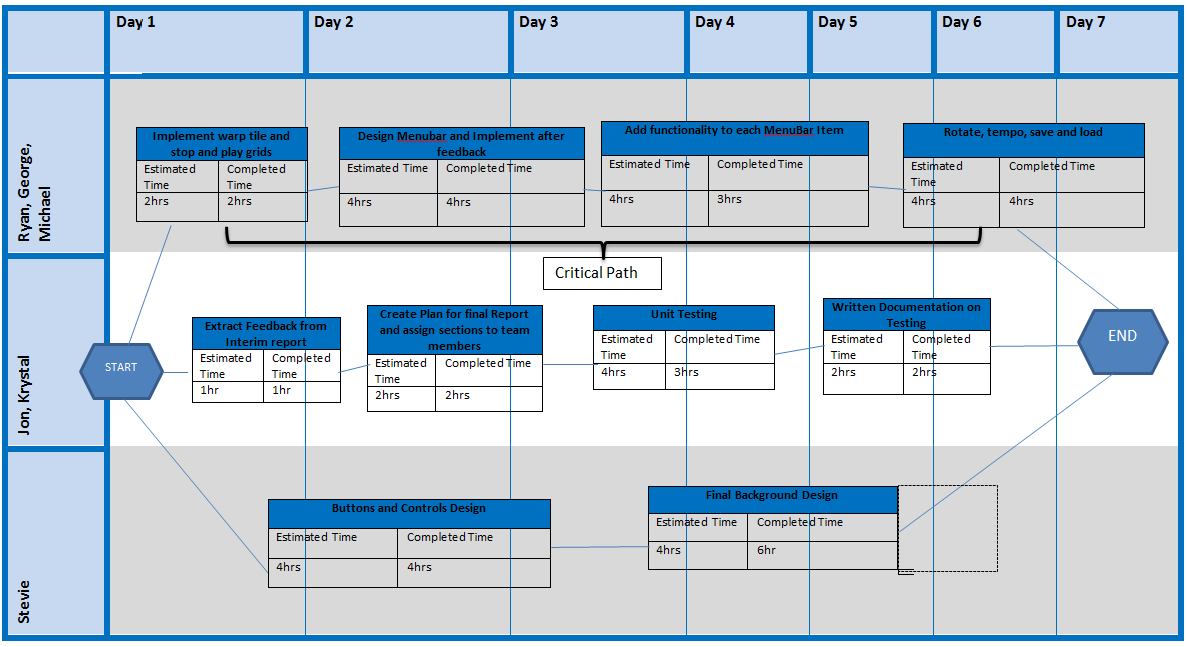
\includegraphics[scale=0.5]{pert.png}\\
\\
We used the tasks that were created at the beginning of the week. The critical path was then identified. The tasks that were on the critical path had to be monitored closely to ensure the successful completion of tasks that week, we did this by keeping in contact daily via Facebook or email or during our weekly group work session. Also during our Monday meetings we reviewed both the pert chart and Kanban boards and checked if we had successfully completed our assigned tasks for that week after this we updated our Gantt to view the overall progress of the project and check if we were on schedule to meet deadlines.\\


\section{Problems Encountered}
Fear of conflict remains to be a constant problem in group working and in our team it was apparent in the early stages of the project. As we were working with each other for the first time nobody wanted to offend each other so opinions on certain matters weren’t challenged and constructive criticism was taken in the wrong way which in turn affected the quality of our initial work. Fear of conflict led to the avoidance of accountability this was because at times the team would refuse to confront difficult issues within the project by avoiding responsibility with the issue at hand and just focus on their given roles. These issues were eradicated with time as the more we worked together the better understanding we had of each other so we were regularly able to provide each other feedback with tasks and also raise any issues if we had any and admit responsibility to some issues . This led to the team being more productive as the focus was working together to produce a high standard of work instead of everyone for their own.\\
\\
Working in a team meant that competency levels within the team differed. For example none of the team had considerable experience in testing. As a result some team members were asked to learn more about J-unit testing and begin writing test cases. Our lack of experience was evident as we weren’t sure which parts of the program needed testing, therefore we didn’t have sufficient test cases for our initial prototypes. This made it difficult for our developer’s to see which part of the code had bugs and needed changes, but after advice from our supervisor and increased proficiency in testing our latest prototype had sufficient test cases. Another issue with different competency levels was that some of the team were working considerably more than others, this was apparent when we were assigning tasks at the beginning of the week, lack of commitment was evident as some would avoid taking responsibility for the harder tasks and just take the smaller ones or even take responsibility for the tasks and not produce their work within the given time. By organising a group working session we were able to help each other stick to task deadlines and motivate each other.\\ 
\\
\part{Conclusion}
It is our conviction that we have produced a project of a high quality and high standard. \textit{'HEX'} conforms to, fulfills and arguably exceeds the specification drawn up at the beginning of the project. Not only have we succesfully emulated the reacTogon hardware, but we have also extended it: affording a truly novel musical experience. The success of the software not only lies in the unique, neoteric functionality and experience; but also in the usability and contemporary design of the user interface. These factors coupled with the quality of the codebase, which employs Java best practice and object-oriented design yields a culmination of our efforts and an ultimately successful project.

\section{References}
\pagebreak

\part{Appendices}
\bibliographystyle{IEEEtran}
\bibliography{reportReferences}

\section{Markey Research Survey}
To be insterted.

\pagebreak
\section{Software Instruction Manual}
TO BE INSERTED SEPARATELY

\pagebreak
\section{Weekly Formal Meeting Minutes}
TO BE INSERTED
\end{document}